\thispagestyle{diendandayvahoctoannone}
\pagestyle{diendandayvahoctoan}
\everymath{\color{diendantoanhoc}}
\graphicspath{{../diendantoanhoc/pic/}}
\blfootnote{$^{1}$\color[named]{diendantoanhoc}Thái Nguyên.}
\begingroup
\AddToShipoutPicture*{\put(0,616){\includegraphics[width=19.3cm]{../bannerdiendan}}}
\AddToShipoutPicture*{\put(44,525){\includegraphics[scale=1]{../tieude2.pdf}}}
\centering
\endgroup
\vspace*{192pt}

Trong bài viết này, tác giả xin giới thiệu với bạn đọc phương pháp sử dụng tiếp tuyến để giải một số bài toán về phương trình, bất phương trình thông qua tính lồi, lõm của hàm số.

\begin{multicols}{2}
	\textbf{\color{diendantoanhoc}$\pmb{1.}$ Khái niệm về tính lồi, lõm và điểm uốn của đồ thị}
	\vskip 0.1cm
	Xét đồ thị $ACB$ của hàm số $y = f(x)$ biểu diễn trong hình dưới đây. Ta giả thiết rằng tại mọi điểm của nó, đồ thị đã cho đều có tiếp tuyến. Tại mọi điểm của cung $AC$ tiếp tuyến luôn luôn ở \emph{phía trên} của $AC$, ta nói $AC$ là một \textbf{\color{diendantoanhoc}\itshape cung lồi}. Nếu $a$ là hoành độ của $A$ và $c$ là hoành độ của $C$ thì khoảng $(a; c)$ được gọi là một khoảng lồi của đồ thị. Tại mỗi điểm của cung $CB$ tiếp tuyến luôn luôn ở \emph{\itshape phía dưới} của $CB$. Ta nói $CB$ là một \textbf{\color{diendantoanhoc}\itshape cung lõm}. Nếu $c$ là hoành độ của $C$, $b$ là hoành độ của $B$ thì khoảng $(c; b)$ được gọi là một khoảng lõm của đồ thị.
	\begin{center}
		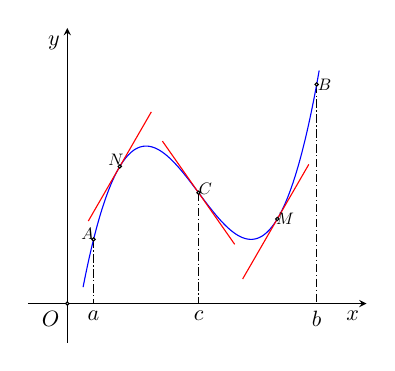
\begin{tikzpicture}
			\def\hsf(#1){((#1)^3-5*(#1)^2+7*(#1)-1}%ham so f
			\draw[-stealth,very thin](-.5,0)--(3.8,0)node[below left,scale=.8]{$x$};%truc Ox
			\draw[-stealth,very thin](0,-.5)--(0,3.5) node[below left,scale=.8]{$y$};%truc Oy
			\draw[fill=white](0,0)circle(.6pt)node[below left,scale=.8]{$O$};%goc toa do O
			\path (1/3,{\hsf(1/3)})coordinate(A) (19/6,{\hsf(19/6)})coordinate(B) (5/3,{\hsf(5/3)})coordinate(C)
			(8/3,{\hsf(8/3)})coordinate(M) (2/3,{\hsf(2/3)})coordinate(N);
			\draw[color=black,densely dash dot, thin] (A)--(1/3,0)node[below ,scale=.8] {$a$} (B)--(19/6,0)node[below ,scale=.8] {$b$} (C)--(5/3,0)node[below ,scale=.8] {$c$};
			\draw[blue,smooth,samples=100] plot[domain=.2:3.2](\x,{\hsf(\x)});
			\draw[red] (C)--+(125:.8)(C)--+(-55:.8) 
			(N)--+(60:.8)(N)--+(-120:.8) 
			(M)--+(60:.8)(M)--+(-120:.88);
			\foreach \p/\g in{A/140,B/0,C/30,M/0,N/120} \draw[fill=white](\p)circle(.6pt)+(\g:.1)node[scale=.6]{$\p$};
		\end{tikzpicture}
	\end{center}
	Điểm phân cách giữa cung lồi và cung lõm được gọi là \textbf{\color{diendantoanhoc}\itshape điểm uốn}. Điểm $C$ của đồ thị trong hình là điểm uốn.
	\vskip 0.1cm
	Nói cách khác thì: 
	Nếu hàm số $y=f(x)$ có đạo hàm trên khoảng $I$ ta nói rằng
	\vskip 0.1cm
	$a)$ Đồ thị ($C$) của hàm số $y = f(x)$ lồi trên khoảng $I$ nếu tiếp tuyến của ($C$) tại mỗi điểm của nó đều nằm phía trên đồ thị.
	\vskip 0.1cm
	$b)$ Đồ thị ($C$) của hàm số $ y = f(x)$ lõm trên khoảng $I$ nếu tiếp tuyến của nó tại mỗi điểm của nó đều nằm phía dưới đồ thị.
	\vskip 0.1cm
	\textbf{\color{diendantoanhoc}Nhận xét:} Một hàm được gọi là lồi (tương ứng, lõm) nếu đồ thị của nó là lồi (tương ứng, lõm). Đồ thị hàm lồi có hình dạng giống như một cái mũ $\cap $ còn của hàm lõm thì có hình dạng giống như một cái cốc  $\cup $.
	\vskip 0.1cm
	\textbf{\color{diendantoanhoc}$\pmb{2.}$ Dấu hiệu lồi, lõm và điểm uốn của đồ thị}
	\vskip 0.1cm
	Ta thừa nhận dấu hiệu lồi, lõm sau đây:
	\vskip 0.1cm
	\textbf{\color{diendantoanhoc}Định lý:} Cho hàm số $y = f(x)$ có đạo hàm đến cấp hai trên khoảng $I$.
	\vskip 0.1cm
	$1)$ Nếu $f "(x)< 0$ với mọi $x\in I$ thì đồ thị của hàm số \textbf{\color{diendantoanhoc}\itshape lồi} trên khoảng đó. 
	\vskip 0.1cm
	$2)$ Nếu $f "(x)> 0$ với mọi $x\in I$ thì đồ thị của hàm số  \textbf{\color{diendantoanhoc}\itshape lõm} trên khoảng đó.
	\vskip 0.1cm
	\textbf{\color{diendantoanhoc}Định lý:} Giả sử hàm số $y = f(x)$ có đạo hàm cấp hai trên một khoảng $I$ chứa điểm $ x _0$. Nếu $f"(x_0) = 0$ và $f"(x) $ đổi dấu khi $x$ qua điểm $x_0$ thì $U(x_0;f(x_0))$ là một điểm uốn của đồ thị hàm số $y = f(x)$.
	\vskip 0.1cm
	Tại điểm uốn tiếp tuyến đi xuyên qua đồ thị.
	\vskip 0.1cm
	\textbf{\color{diendantoanhoc}$\pmb{3.}$ Điều kiện để hai đường cong tiếp xúc nhau}
	\vskip 0.1cm
	Điều kiện để hai đường cong $y= f(x)$ và $y=g(x) $ tiếp xúc nhau là hệ phương trình sau có nghiệm và nghiệm của hệ là hoành độ giao điểm của hai đường cong đó \begin{align*}
		\begin{cases}f(x)=g(x)\\ f'(x)=g'(x)\end{cases}\tag{$*$}
	\end{align*}
	Vậy, đồ thị của $f$ và $g$ tiếp xúc nhau tại $x_0$ khi và chỉ khi $x_0$ là nghiệm của hệ ($*$).
	\vskip 0.1cm
	Thêm vào đó, nếu hai đường cong $y=f(x)$ và $y=g(x)$ có tính lồi lõm trái ngược nhau, ngoài ra có chung nhau tiếp tuyến thì khi đó phương trình $f(x)=g(x)$ có nghiệm duy nhất.
	\begin{center}
		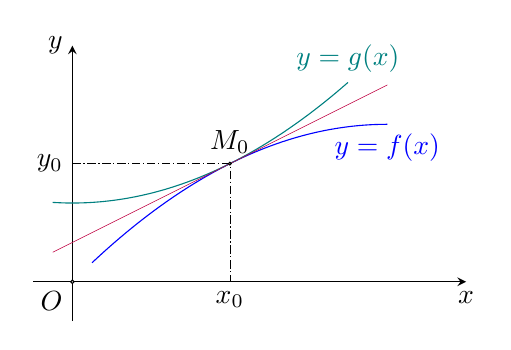
\begin{tikzpicture}
			\def\hsf(#1){-.125*(#1)^2+(#1)}%ham so f
			\def\hsg(#1){.125*(#1)^2+1}%ham so g
			\draw[-stealth] (-.5,0)--(5,0)node[below]{$x$};
			\draw[-stealth] (0,-.5)--(0,3)node[left]{$y$};
			\draw[fill=white](0,0)circle(.6pt)node[below left]{$O$};
			\draw[densely dash dot,very thin] (0,3/2)node[left]{$y_0$}-|(2,0) node[below]{$x_0$};
			\draw[smooth,blue]plot[domain=.25:4](\x,{\hsf(\x)}) node[below]{$y=f(x)$};
			\draw[smooth,teal]plot[domain=-.25:3.5](\x,{\hsg(\x)}) node[above]{$y=g(x)$};
			\draw[smooth,very thin,purple]plot[domain=-.25:4](\x,{.5*\x+1/2});
			\draw[fill=white](2,3/2)circle(.5pt)node[above]{$M_0$};
		\end{tikzpicture}
	\end{center}
	Cần phải chú ý rằng nhiều tài liệu trong và ngoài nước hiện nay định nghĩa về tính lồi (convex), lõm (concave) của đồ thị hàm số khác như đã nêu ở trên. Cụ thể là hàm lồi trong bài viết này được gọi là hàm lõm trong một số tài liệu, còn hàm lõm trong bài viết này thì lại được họ gọi là hàm lồi. 
	\vskip 0.1cm
	\textit{\textbf{\color{diendantoanhoc}Ta sẽ vận dụng những tính chất và nhận xét trên để ứng dụng trong việc giải một số bài toán về phương trình, bất phương trình, đây cũng chính là cở sở của phương pháp tiếp tuyến trên}}.
	\vskip 0.1cm
	Trong bài viết này chúng ta viết tắt VT cho vế trái, VP cho vế phải.
	Việc kiểm tra dấu hiệu lồi, lõm của hàm số bằng cách tính đạo hàm cấp hai trong một số ví dụ sẽ được dành cho bạn đọc.
	\vskip 0.1cm
	\textbf{\color{diendantoanhoc}$\pmb{4.}$ Các ví dụ}
	\vskip 0.1cm
	\textbf{\color{diendantoanhoc}Ví dụ $\pmb{1.}$} Giải phương trình
	\begin{align*}
		x^2-2x+5=\sqrt{x+3}+\sqrt{5-x}.
	\end{align*}
	\textit{Lời giải.} Điều kiện $-3\leq x\leq 5$. Vế trái là hàm lõm còn vế phải là hàm lồi (bạn đọc tự kiểm tra), chúng có chung tiếp tuyến tại $(1;4)$. Vậy $x=1$ là nghiệm duy nhất của phương trình.
	\vskip 0.1cm
	\textbf{\color{diendantoanhoc}Nhận xét:} Bài tập kiểu như trên rất quen thuộc với nhiều bạn đọc, phương pháp thường dùng là đánh giá bất đẳng thức. Ở đây, chúng ta sử dụng tiếp cận khác thông qua tiếp tuyến.
	\vskip 0.1cm
	Ta sẽ đến với những ví dụ khác, đòi hỏi đến cả kỹ năng nhẩm nghiệm.
	\vskip 0.1cm
	\textbf{\color{diendantoanhoc}Ví dụ $\pmb{2.}$} Giải phương trình
	\begin{align*}
		\sqrt[6]{6x-5}=\dfrac{x^{7}}{8x^{2}-10x+3}.
	\end{align*}
	\textit{Lời giải.} Điều kiện $x\ge \frac{5}{6}$. Với $x\ge \frac{5}{6}$ thì $VT$ là hàm lồi, liên tục, vì vậy đồ thị hàm số nằm dưới tiếp tuyến của nó tại điểm $x=1$ là $y=x+1$.
	Với $x\ge\frac{5}{6}$ thì $VP$ là hàm lõm, liên tục, vì vậy đồ thị hàm số nằm trên tiếp tuyến của nó tại điểm $x=1$ là $y=x+1$.
	\vskip 0.1cm
	Vậy $x=1$ là nghiệm duy nhất của phương trình. 
	\vskip 0.1cm
	\textbf{\color{diendantoanhoc}Ví dụ $\pmb{3.}$} Cho hai hàm số $f(x)$ và $g(x)$ được xác định như sau: $f(x)=\sqrt{13x^{2} - 6x + 10 } + \sqrt{5x^{2} -13x + \frac{17}{2}} + \sqrt{17x^{2} - 48x + 36} $ và $g(x)= \dfrac{1}{2}(36x - 8x^{2} - 21)$.
	\vskip 0.1cm
	Giải phương trình $f(x)=g(x)$.
	\vskip 0.1cm
	\textit{Lời giải.} Điều kiện $x\in \mathbb R$. Đặt $h(x)=f(x)-g(x)$\\ Không khó để chỉ ra $h(x)$ là hàm lõm, liên tục. Nhận thấy $h(\dfrac{3}{2})=0$ và $h'(\dfrac 32)=0$ , do đó đồ thị hàm số tiếp xúc với trục hoành tại điểm $x=\dfrac{3}{2}$.
	\vskip 0.1cm
	Vậy $x=\dfrac{3}{2}$ là nghiệm duy nhất của phương trình của bài toán.
	\vskip 0.1cm
	\textbf{\color{diendantoanhoc}Ví dụ $\pmb{4.}$} Giải phương trình
	\begin{align*}
		x\sqrt{x^2\!+\!6}\!+\!(x\!+\!1)\sqrt{x^2\!+\!2x\!+\!7}\!=\!\dfrac{13}{5}(2x\!+\!1)
	\end{align*}
	\textit{Lời giải.}  Điều kiện $x\in\mathbb R$. Đặt $g(x)=x\sqrt{x^2+6}$ và $f(x)=g(x+1)+g(x)$.
	\vskip 0.1cm
	Ta dễ kiểm tra thấy rằng:
	\vskip 0.1cm
	$a)$ $g(x)$ là hàm lẻ và $g''(x)$ cũng là hàm lẻ; hơn nữa ta cũng có $f(-\dfrac 12)=f''(-\dfrac 12)=0$.
	\vskip 0.1cm
	$b)$ $g(x)$ và $g''(x)$ là hàm đồng biến, suy ra $f(x)$ và $f''(x)$ cũng là hàm đồng biến.
	\vskip 0.1cm
	$c)$ Tiếp tuyến với đồ thị của hàm số  $f(x)$ tại $x=-\dfrac 12$ là $y=\dfrac{13}5(2x+1)$.
	\vskip 0.1cm
	Vậy đồ thị hàm số $f(x)$ nằm dưới tiếp tuyến của nó khi $x<-\dfrac 12$ và đồ thị hàm số $f(x)$ nằm trên tiếp tuyến của nó khi $x>-\dfrac 12$.
	\vskip 0.1cm
	Vậy $x=-\dfrac{1}{2}$ là nghiệm duy nhất của phương trình.
	\vskip 0.1cm
	\textbf{\color{diendantoanhoc}Chú ý:} Ở ví dụ này nghiệm của phương trình chính là hoành độ điểm uốn của đồ thị.
	\vskip 0.1cm
	\textbf{\color{diendantoanhoc}Ví dụ $\pmb{5.}$} Giải phương trình
	\begin{align*}
		&3\left(x^{3}+\frac{x}{\sqrt{\left(1+x^{2} \right)^{3}}} \right)+2\\
		=\,\,&\sqrt{\left(1+x \right)^{3}}+\sqrt{\left(1-x \right)^{3}}.
	\end{align*}
	\textit{Lời giải.}  Điều kiện xác định $x\in[-1;1]$. Nhận xét rằng $x=0$ là một nghiệm của phương trình. Đặt $f(x)=x+(1+x)^{-\frac 32}$ và $g(x)=\dfrac{(1+x)^{\frac 32}+(1-x)^{\frac 32}-2}x$.
	\vskip 0.1cm
	Giả sử $x\ne 0$. Phương trình đã cho có thể được viết lại thành $3f(x^2)=g(x)$.
	\vskip 0.1cm
	Chú ý rằng:
	\vskip 0.1cm
	Một mặt, $g(x)$ là hàm lẻ, nhận giá trị âm trên $[-1;0)$ và dương trên $(0, 1]$ và đồng biến trên mỗi khoảng này (bạn đọc tự kiểm tra), nên $g(x)\le g(1)=2\sqrt 2-1 <1$ với mọi $0\ne  x\in[-1,1]$.
	\vskip 0.1cm
	Mặt khác, $f(x)$ là hàm lõm trên $[0,1]$ (bạn đọc tự kiểm tra), vì vậy đồ thị hàm số nằm trên tiếp tuyến của nó tại điểm $x=0$ : $f(x)\ge 1-\frac x2\ge \frac 12$.
	\vskip 0.1cm
	Vậy $f(x^2)\ge \frac 12$, suy ra $3f(x^2)\ge \frac 32 > 1\ge g(x)$, do đó phương trình không còn nghiệm nào nữa. 
	\vskip 0.1cm
	Vậy $x=0$ là nghiệm duy nhất của phương trình đã cho.
	\vskip 0.1cm
	\textbf{\color{diendantoanhoc}Ví dụ $\pmb{6.}$} Cho số lẻ $n>1$. Giải phương trình
	\begin{align*}
		n^{x^n-1}+n^{\frac{1}{x}}=n+1.
	\end{align*}
	\textit{Lời giải.} Điều kiện xác định: $x \neq 0$. 
	Nếu $x<0$ thì VT$<2<$VP nên trường hợp này phương trình vô nghiệm.
	\vskip 0.1cm
	Xét trường hợp $x>0$. Xét hàm số $f(x):\mathbb R^+\to \mathbb R$ xác định bởi:
	\begin{align*}
		f(x)=n^{x^n-1}+n^{\frac 1x}-n-1
	\end{align*}
	Ta lần lượt có:
	\begin{align*}
		f'(x)=&\,n(\ln n)x^{n-1}n^{x^n-1}-\frac {\ln n}{x^2}n^{\frac 1x}.\\
		f''(x)=&\,n(\ln n)\left(n(\ln n)x^{2n-2}+(n-1)x^{n-2}\right)\\
		&\times n^{x^n-1}+\ln n\left(\frac {\ln n}{x^4}+\frac 2{x^3}\right)n^{\frac 1x}.
	\end{align*}
	Nhận thấy rằng $f(1)=f'(1)=0$, do đó tiếp tuyến của hàm số $f(x)$ tại điểm $x=1$ là trục hoành.
	\vskip 0.1cm 
	Vì $f(x)$ là hàm lõm và liên tục ($f''(x)>0$) do đó $x=1$ là nghiệm duy nhất của phương trình. 
	\vskip 0.1cm
	\textbf{\color{diendantoanhoc}Ví dụ $\pmb{7.}$} Giải bất phương trình
	\begin{align*}
		45x^3\!-\!17x^2\!-\!37x\!+\!25\!\ge\! 4\sqrt{\!\!(x\!+\!1)(5x\!-\!3)^3}.
	\end{align*}
	\textit{Lời giải.} Bất phương trình đã cho được viết lại thành 
	\begin{align*}
		(x\!+\!1\!)(45x^2\!-\!62x\!+\!25)\!\ge\! 4\sqrt{\!\!(x\!+\!1\!)(5x\!-\!3)^3}.
	\end{align*}
	Nhận thấy rằng một nghiệm là $x=-1$; các nghiệm khác phải thỏa mãn $x>-1$ (trái lại thì VT$<0\le$ VP), và thật ra $x\ge\frac 35$ (trái lại thì VP không xác định).
	\vskip 0.1cm
	Khi đó (với điều kiện $x\ge\frac 35$) bất phương trình trở thành
	\begin{align*}
		45x^2-62x+25\ge 4(5x-3)\sqrt{\dfrac{5x-3}{x+1}}.
	\end{align*}
	Nhận thấy một nghiệm thứ hai là $x=\frac 35$. Vậy với $x>\frac 35$ bất phương trình trở thành
	\begin{align*}
		\dfrac{45x^2-62x+25}{4(5x-3)}\ge \sqrt{\dfrac{5x-3}{x+1}}.
	\end{align*}
	VT là hàm lõm (bạn đọc tự kiểm tra) với tiếp tuyến $y=x$ tại $x=1$, VP là hàm lồi (bạn đọc tự kiểm tra) với tiếp tuyến $y=x$ tại $x=1$. Vậy đồ thị hàm số VT luôn nằm trên đồ thị của VP,  do đó bất phương trình luôn đúng.
	\vskip 0.1cm
	Vậy nghiệm của bất phương trình là: \linebreak $x\in\{-1\}\cup\left[\frac 35,+\infty\right)$
	\vskip 0.1cm
	\textbf{\color{diendantoanhoc}$\pmb{5.}$ Bài tập đề nghị}
	\vskip 0.1cm
	\textbf{\color{diendantoanhoc}Bài $\pmb{1.}$} Giải các phương trình sau trên tập số thực
	\vskip 0.1cm
	$a)$  $\sqrt[4]{x}=\frac{3}{8}+2x$.
	\vskip 0.1cm
	$b)$ $8x^2+\sqrt{\frac{1}{x}}=\frac{5}{2}.$
	\vskip 0.1cm
	$c)$ $16x^4+5=6\sqrt[3]{4x^3+x}.$
	\vskip 0.1cm
	$d)$ $ 2\sqrt[4]{\dfrac{x^{2}}{3}+4}=1+\sqrt{\dfrac{3x}{2}}.$
	\vskip 0.1cm
	$e)$ $x^2+2x+4=3\sqrt{x^3+4x}.$
	\vskip 0.1cm
	$f)$ $2^{x^2}+3^{x^2}+4^{x^2}+5^{x^2}=4^{1-x^2}.$
	\vskip 0.1cm
	$g)$ $x^2+x = (6x-x^2-2)\sqrt{x-1}.$
	\vskip 0.1cm
	$h)$ $2x^2-11x+21-3\sqrt[3]{4x-4}=0.$
	\vskip 0.1cm
	$i)$ $x^{3}+x^{2}-15x+30=4\sqrt[4]{27(x+1)}.$
	\vskip 0.1cm
	$j)$ $2\sqrt[4]{27x^2+24x+\frac{28}{3}}=1+\sqrt{\frac{27x}{2}+6}.$
	\vskip 0.1cm
	$k)$ $\sqrt{x^2+x-1}+\sqrt{x-x^2+1}=x^2-x+2.$
	\vskip 0.1cm
	$l)$ $x^2-2x+3=\sqrt{2x^2-x}+\sqrt{1+3x-3x^2}.$
	\vskip 0.1cm
	$m)$ $\sqrt{x^2+x+19}+\sqrt{7x^2+22x+28}$\\
	$\quad\,\,+\sqrt{13x^2+43x+37}=3\sqrt{3}(x+3)$.
	\vskip 0.1cm
	$n)$ $\log_2 \dfrac{2x+1}{4x} = \log_{x} \dfrac{2x+1}{2}.$\\
	\vskip 0.1cm
	\textbf{\color{diendantoanhoc}Bài $\pmb{2.}$} Tồn tại hay không các cặp số thực âm $(x,y)$ thoả mãn phương trình \linebreak$x2^y+y2^{-x}=x+y$?
	\vskip 0.1cm
	\textbf{\color{diendantoanhoc}Bài $\pmb{3.}$} Tìm tất cả các số thực $a$ sao cho bất phương trình $a^x\geq 1+x\log _{11}12$ đúng với mọi số thực $x$.
	\vskip 0.1cm
	\textbf{\color{diendantoanhoc}Tài liệu tham khảo}
	\vskip 0.1cm
	[$1$] Ngô Thúc Lanh (chủ biên), {\it Giải tích $12$ }(SGK), Nhà xuất bản Giáo Dục ($2006$).
	\vskip 0.1cm
	[$2$] Nguyễn Huy Đoan (chủ biên), {\it Giải tích $12$ nâng cao} (SGK), Nhà xuất bản Giáo Dục ($2008$).
	\vskip 0.1cm
	[$3$] Phan Đức Chính (chủ biên), {\it Một số phương pháp chọn lọc giải các bài toán sơ cấp (Tập $2$)}, Nhà xuất bản Đại học Quốc gia Hà Nội ($2003$). 
	\vskip 0.1cm
	[$4$] Nguyễn Quang Nam, {\it Kỹ thuật tạo nhân tử kép}, Tạp chí Toán học và Tuổi trẻ, Nhà xuất bản Giáo Dục (Số $511$, tháng $1/2020)$.
	\vskip 0.1cm
	[$5$]~\url{https://artofproblemsolving.com/com} \url{munity}
	\end{multicols}